%%%%%%%%%%%%%%%%%%%%%%%%%%%%%%%%%%%%%%%%%%%%%%%%%%%%%%%%%%%%%%%%%%%%%%%%
%%%%%                                                              %%%%%
%%%%% Chapter 3: SMURF-seq                                         %%%%%
%%%%%                                                              %%%%%
%%%%%%%%%%%%%%%%%%%%%%%%%%%%%%%%%%%%%%%%%%%%%%%%%%%%%%%%%%%%%%%%%%%%%%%%
\chapter{Sampling molecules using re-ligated fragments (SMURF)-seq}
\label{ch3}


%%%%%%%%%%%%%%%%%%%%%%%%%%%%%%%%%%%%%%%%%%%%%%%%%%%%%%%%%%%%%%%%%%%%%%%%
%%%%%%%%%%%%%%%%%%%%%%%%%%%%%%%%%%%%%%%%%%%%%%%%%%%%%%%%%%%%%%%%%%%%%%%%
%%%%%%%%%%%%%%%%%%%%%%%%%%%%%%%%%%%%%%%%%%%%%%%%%%%%%%%%%%%%%%%%%%%%%%%%
\section{Naive approaches to read-counting on nanopore machines}
%% Long read approach
Copy number profiling, and read-counting in general, can be done on
nanopore sequencers with long reads ($\sim$8kb) following the standard
sequencing procedure.
% Advantages of long read sequencing
Since nanopore machines are optimized for long read sequencing, this
method has the advantage of using any standard library preparation
protocol that are commercially available.  Sequencing these long
molecules using a nanopore keeps a pore occupied for a longer duration
once a pore is loaded followed by an open pore waiting for a molecule to
be reload in a pore.  Further, technical nucleotides, such as sequencing
adapters and barcodes, are sequenced one (or twice) every $\sim$8k
bases, thus the fraction of time a nanopore spends sequencing technical
nucleotides is low.
% Disadvantages of long read sequencing
However, read-counting applications do not benefit from longer reads
beyond what is necessary for unique mapping to the reference genome. In
these applications, for any fixed number of nucleotides sequenced, more
information would be obtained if those nucleotides are organized as more
DNA molecules, rather than longer contiguous fragments.

%% Short read sequencing
An alternate approach to read-counting is to sequence short reads
($\sim$150 bp) directly on a nanopore sequencer.
%% Advantages of short read sequencing
In general, for a given sample of DNA, a nanopore instrument will
generate more reads if the corresponding molecules are shorter.  Once a
molecule is loaded into a pore, the time spent sequencing is less for
shorter reads. In addition, for a fixed amount of DNA, shorter molecules
result in higher molar concentration when loaded onto the machine,
increasing the rate at which each pore captures molecules
\citep{muthukumar2010theory,wanunu2008dna}. Therefore, sequencing short
reads on a nanopore machine would generate more reads from a sequencing
run than sequencing long reads.
%% Disadvantages of short read sequencing
However, sequencing short reads requires ad-hoc modifications to the
library preparation protocol as these are optimized for longer
molecules.  Sequencing these shorter molecules keeps a pore occupied for
a shorter duration once a pore is loaded followed by waiting for a pore
to be reloaded (but the reload time is usually shorter due to the higher
molar concentration) Moreover, technical nucleotides are sequenced every
$\sim$150bp, increasing the fraction of time a nanopore sequences the
technical bases.

\begin{figure}[t!]
\centering
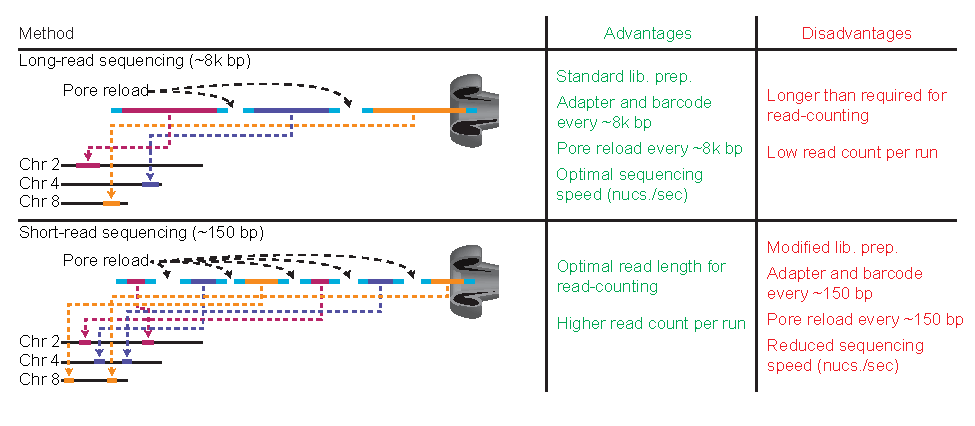
\includegraphics{naive_counting.pdf}
\caption[Naive approaches to read-counting on nanopore machines]{
  Naive approaches to read-counting on nanopore machines.
  Sequencing long-reads directly is optimized for nanopore machines but
  not for read-counting applications.
  Sequencing short-read is optimized for read-counting applications but
  not for nanopore sequencing.}
\label{smurf}
\end{figure}

%% SMURF-seq approach
SMURF-seq approach combines the advantages of both of these methods
while alleviating the drawbacks by using a nanopore instrument as
intended for long-read sequencing, while generating the desired short
fragments. Using the SMURF-seq approach we generate higher read counts
per run than sequencing long or short molecules directly.


%%%%%%%%%%%%%%%%%%%%%%%%%%%%%%%%%%%%%%%%%%%%%%%%%%%%%%%%%%%%%%%%%%%%%%%%
%%%%%%%%%%%%%%%%%%%%%%%%%%%%%%%%%%%%%%%%%%%%%%%%%%%%%%%%%%%%%%%%%%%%%%%%
%%%%%%%%%%%%%%%%%%%%%%%%%%%%%%%%%%%%%%%%%%%%%%%%%%%%%%%%%%%%%%%%%%%%%%%%
\section{SMURF-seq approach to read counting}
%% SMURF-seq concept
The SMURF-seq protocol involves cleaving genomic DNA into short
fragments, with length just sufficient for an acceptable rate of
uniquely mapping fragments in the reference genome.  These fragmented
molecules are then randomly ligated back together to form artificial
long DNA molecules, as required for long-read sequencing. The long
re-ligated molecules are sequenced following the standard MinION library
preparation protocol. After (or possibly concurrent with) sequencing,
the SMURF-seq reads are mapped to the reference genome in a way that
simultaneously splits them into their constituent fragments, each
aligning to a distinct location in the genome (Fig.~\ref{smurf}).

\begin{figure}[b!]
\centering
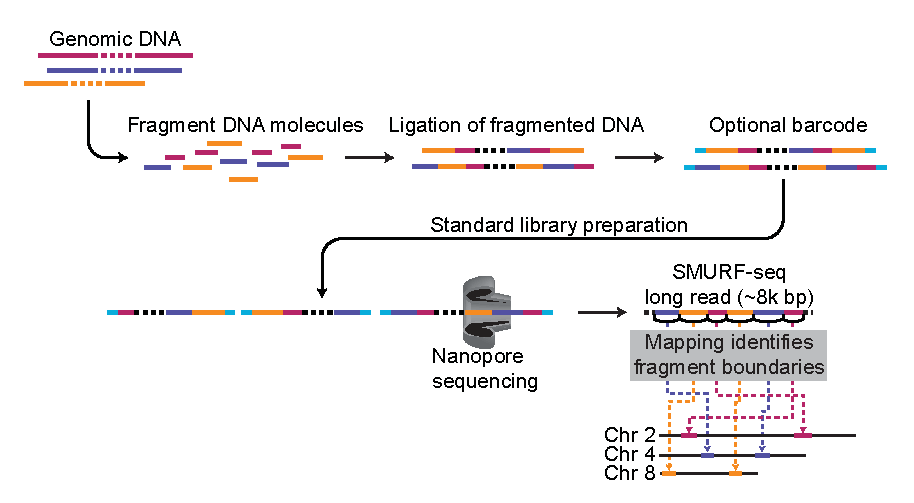
\includegraphics{smurf.pdf}
\caption[SMURF-seq approach to sequencing short fragments]{
  SMURF-seq approach to sequencing short fragments.
  SMURF-seq efficiently sequences short fragments of DNA for
  read-counting applications with a reference genome on long-read
  sequencers, and yields up to 30 countable fragments per sequenced read.
  SMURF-seq sequences short DNA molecules by generating long concatenated
  molecules from these.  SMURF-seq reads are aligned by splitting them
  into multiple fragments, each aligning to a distinct region in the
  genome.}
\label{smurf}
\end{figure}


\begin{figure}[t!]
\centering
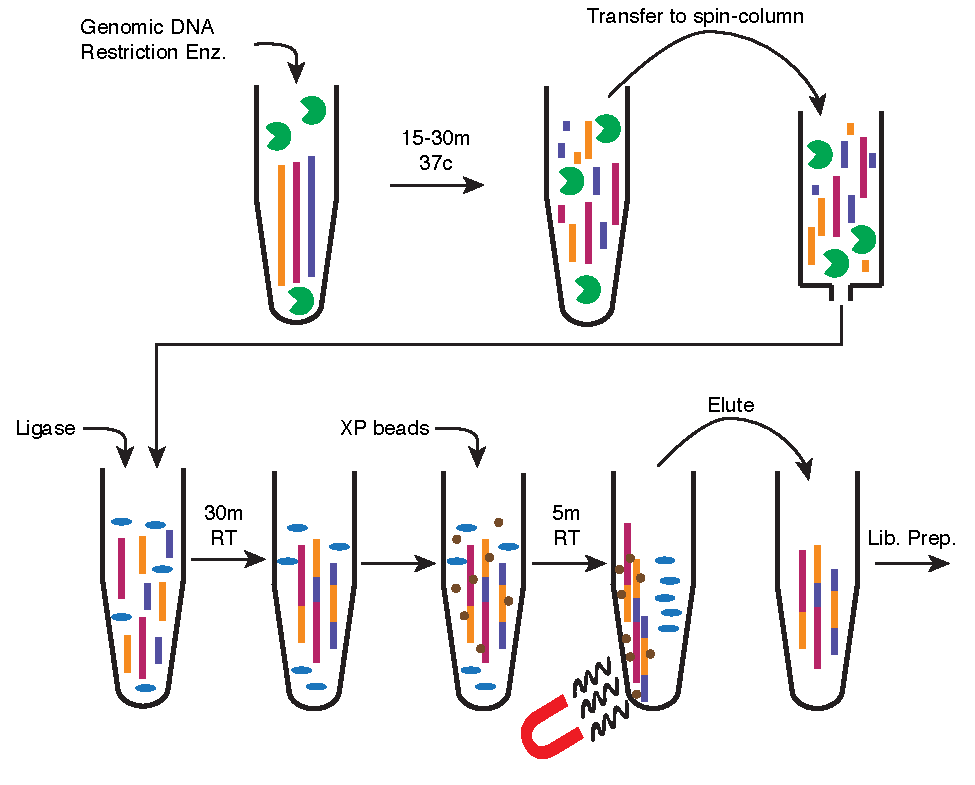
\includegraphics{ch3_fig2.pdf}
\caption[Schematic of SMURF-seq protocol]{
  Schematic of SMURF-seq protocol. SMURF-seq consists of four
  steps: restriction enzyme digestion, spin-column clean-up, re-ligation
  of fragmented DNA, and Ampure XP beads clean-up.}
\label{protocol}
\end{figure}

%% Description of SMURF-seq protocol
More specifically, genomic DNA was fragmented using restriction enzymes
and ligated with T4 DNA ligase, with clean-up steps in between.
SMURF-seq protocol is completely enzymatic and takes less than 90
minutes to complete (Fig.~\ref{protocol}).  The details of these steps
are given below:
%%
\begin{enumerate}
\item Restriction enzyme digestion: restriction enzymes recognize
  and cleave specific DNA sequences, typically producing sticky-ended DNA
  molecules.
  %% choice of re used
  The choice of restriction enzyme used is primarily dependent on the
  size of the fragmented molecules produced. Based on the downstream
  application, they could also be influenced by other factors such as any
  bias they could introduce.
  %% advantages
  An advantage of using restriction enzymes to fragment DNA molecules,
  over other fragmentation techniques, is that the fragmented molecules
  have a uniform ends (either overhangs with the same sequence or
  blunt-ends) and are thus compatible for ligation without an end-repair
  step in between.

\item Clean-up: the reaction containing the restriction
  enzymes and the fragmented DNA molecules is cleaned to wash out the
  enzymes and retain the DNA molecules. The choice of clean-up kit used, also
  determines the length of the DNA molecules that are retained. We used a
  spin-column based clean-up that typically retains molecules that are over
  $\sim$70 bp. However, other clean-up kits, such as bead-based kits,
  could also be used at this step.

\item Re-ligation: fragmented DNA molecules with uniform ends are
  ligated at random with T4 DNA ligase enzymes.
  %% influence of time
  The most important factor in a ligation reaction is the
  concentration of compatible DNA ends \citep{dugaiczyk1975ligation}. At
  high concentrations, the chances are higher for ligation between two
  molecules than a molecule self-ligating. At low concentrations, the
  chances are higher for self-ligation.
  %%
  Thus, the main consideration during the ligation step is the
  duration of the ligation reaction, as the molar concentration of DNA
  molecules decrease with time. Too little time would lead to insufficient
  ligation, resulting in molecules of length that do not achieve optimal
  SMURF-seq efficiency. On the other extreme, too much time would result
  in circular molecules that are incompatible with the most downstream
  library preparation process. A typical ligation reaction would contain
  both short and circularized molecules, and achieving a balance between
  these determines the efficiency of SMURF-seq.
  %%
  Other factors such as the temperature and buffer contents also affect
  the ligation process.
  %% our experiments
  In our experiments, the ligation reaction was performed at a DNA
  concentration of \SI{25}{\nano\gram}$/$\SI{}{\micro\litre}
  (\SI{500}{\nano\gram} of DNA in \SI{10}{\micro\litre} nuclease free
  water and \SI{10}{\micro\litre} DNA ligase) for \SI{30}{\minute}.

\item Bead-based clean-up: the reaction containing the ligase enzymes and
  ligated DNA molecules is cleaned to retain only the ligated molecules. We
  used a bead-based clean-up at this step to avoid damage to long DNA
  molecules that are typical of spin-column based methods.
\end{enumerate}

%% Library construnction using standard protocols
DNA molecules that are resultant of the SMURF-seq protocol are long DNA
molecules that are several kilo-bases long, and therefore, any standard
library preparation kits that are available for nanopore machines can be
used with SMURF-seq molecules. These molecules can also be barcoded
with one (or two) barcode sequences per molecule. Thus, the SMURF-seq
approach overcomes the disadvantages of sequencing long or short DNA
molecules directly on a nanopore machine for read-counting applications,
and improves its efficiency for read-counting applications.

We also tested dsDNA Fragmentase enzymes (New England Biolabs) and
acoustic shearing (Covaris) to fragment DNA. However, these methods
require an additional end-repair step after fragmentation and the
ligated molecules failed to reach the lengths we obtained by using
restriction fragmentation.

\begin{figure}[t!]
\centering
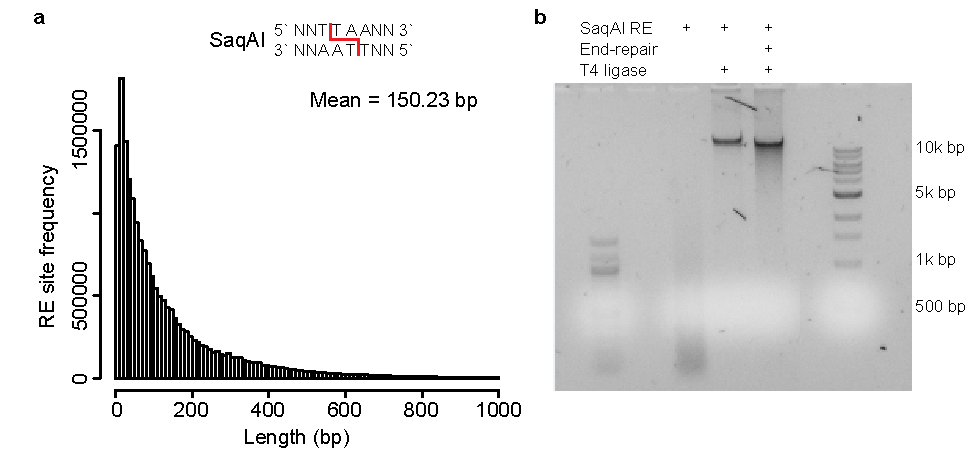
\includegraphics{ch3_fig3.pdf}
\caption[Restriction digestion and ligation of DNA molecules.]{
  Restriction digestion and ligation of DNA molecules.
  (a) Distribution of length between restriction sites computed
  by measuring the distance between the recognition sites on the human
  reference genome. SaqAI recognizes the sequence TTAA and leaves a 2 bp
  overhang.
  (b) Negative gel image of fragmented and ligated normal diploid DNA
  using SaqAI restriction enzyme and T4 DNA ligase.  Sticky-end and
  blunt-end ligation (by end-repair) of fragmented DNA are shown, and
  both yield ligated molecules of approximately the same length.}
\label{re_frag}
\end{figure}

%% The sepecifics of our experiment
%% restriction digestion
In our applications, we used SaqAI restriction enzyme, which recognizes
the sequence TTAA and produces molecules with mean lengths of 150.2 bp
(Fig.~\ref{re_frag}a).
%% re-ligation
The fragmented DNA molecules are then ligated randomly to form longer
molecules using T4 DNA ligase enzyme (Fig.~\ref{re_frag}b).
%
In our experiments, the resulting long DNA molecules were sequenced
using the Oxford Nanopore Technologies 1D DNA by ligation kit
(SQK-LSK108) or the rapid sequencing kit (SQK-RAD003) following the
standard manufacturers protocol. We also multiplexed samples using the
1D native barcoding genomic DNA kit (EXP-NBD103) followed by library
preparation using the 1D DNA by ligation kit.
%
The detailed SMURF-seq protocol is given in Appendix~\ref{appendA}.


%%%%%%%%%%%%%%%%%%%%%%%%%%%%%%%%%%%%%%%%%%%%%%%%%%%%%%%%%%%%%%%%%%%%%%%%
%%%%%%%%%%%%%%%%%%%%%%%%%%%%%%%%%%%%%%%%%%%%%%%%%%%%%%%%%%%%%%%%%%%%%%%%
%%%%%%%%%%%%%%%%%%%%%%%%%%%%%%%%%%%%%%%%%%%%%%%%%%%%%%%%%%%%%%%%%%%%%%%%
\section{Mapping SMURF-seq reads}
The reads sequenced using SMURF-seq can be mapped to a reference genome
by first identifying short matches within the reads, corresponding to
parts of the individual fragments, and then extending those to locate
fragment boundaries.
%
As currently implemented, SMURF-seq fragments are longer than
$\sim$150bp, and mapping these reads is is handled nicely using the
seed-and-extend paradigm implemented in many existing long-read mapping
tools. Although none of these tools were designed to align SMURF-seq
reads, several long read aligners include steps designed for split-read
alignment, which can be leveraged from aligning SMURF-seq reads.

%% TODO: Need to expand on the four steps below
Aligning SMURF-seq reads with long-read mapping tools involve variations
of the following steps:
%% Steps involved in mapping SMURF-seq reads
\begin{itemize}
\item Identifying seeds: Mapping tools have a step of identifying seeds,
  which are short exactly matching parts of the read with parts of the
  reference genome. Choices in how seeds are defined and used are often
  made for mapping speed. The total size of SMURF-seq data sets is
  currently (relatively) small, so speed is not our primary concern. We
  favor the most sensitive seed strategy, but depending on implementation
  too many seed hits could lead to ambiguity later in the mapping process.
\item Chaining seeds: The identified seeds are further extended into
  proto alignments, and filtered to avoid aligning potentially false
  positive seed hits.
\item Aligning within the chains: In this stage a Smith-Waterman
  alignment is performed, typically allowing users to specify a mismatch
  penalty along with penalties for both gap-open and gap-extend.
\item Selecting best alignments: When high-scoring alignments overlap
  within a read, one of them (or both) could be trimmed or one is selected
  and the other discarded. The choices made here could lead to discarding
  entire fragments.
\end{itemize}

%% parameter options
Mapping tools have several parameter options, in general, these are
related to: (1) the seeding and chaining algorithm used by the
individual tool.  (2) The Smith-Waterman alignment scores, i.e. the
match score, and the mismatch and indel penalty. The seeding and
chaining parameters control the number of proto alignments that are
further refined by aligning parts of the read to the reference genome
using the specified alignment scores.

%% Importance of picking the optimal SW score
The Smith-Waterman alignment score used to align fragments to the
reference genome is crucial for determining the optimal fragment length.
On one extreme, a match score of 1 with a mismatch and indel penalty of
0 will result in one identified fragment covering the entire read and
mapping perfectly, but will always map ambiguously. On the other
extreme, a match score of 1 with a mismatch and indel penalty of
$-\infty$ will result in any mismatch or indel on the read to be
considered as a fragment boundary. Therefore to align SMURF-seq reads,
we need to determine optimal alignment scores to use.

We evaluated mapping tools on simulated SMURF-seq data generated by
concatenating random fragments from real Oxford Nanopore reads. This
emulates idealized SMURF-seq reads. Within the simulated reads, the
boundaries of each fragment are known \textit{a priori}, as are their
mapping locations when in the context of their original long reads. We
used this information to evaluate mapping tools in terms of (1) how well
they identify fragments purely for the purpose of counting molecules,
which is the primary information used in CNV analysis, and (2) how well
they identify individual mapping bases within reads. After mapping these
reads, we calculated precision and recall for identifying both the
correct fragment locations, and the individual mapping bases within the
fragments (i.e. the correct fragment boundaries). Using this simulation
setup, we determined the optimal Smith-Waterman alignment score for use
with SMURF-seq reads.

\subsection{Simulating SMURF-seq reads to evaluate mapping programs}
To test these mapping tools, we chose to create simulated reads with the
technical characteristics we expect in idealized SMURF-seq data. We
first selected a fragment length $\ell$ and a number $k$ of fragments
per read. Then, for a given WGS nanopore data set, we took the set of
mapped long reads as determined by BWA-MEM (with \texttt{-x ont2d}
option).
Each of the mapped reads was split into fragments of length $\ell$ (with
a random offset of $0$ to $\ell-1$ at the start of the long read). Each
fragment was validated by requiring that it did not overlap a deadzone
in the genome (as determined by the deadzone program available from
https://github.com/smithlabcode/utils for 40 bp). The reason for
excluding deadzones is that even when a short fragment has a ``known''
mapping location when it is part of a longer read, we cannot compare its
reported mapping location as a short fragment with that known location,
since we expect any good mapping algorithm to identify that the fragment
maps ambiguously. Among these validated fragments, subsets of $k$ were
sampled uniformly at random and concatenated (in random order and
orientation) to form simulated SMURF-seq reads.

The first and last fragments in a read should be slightly easier to
identify and map than the rest, since one of their boundaries is
known. Using the above procedure, we select $k=20$ so that the
simulated reads have a sufficient number of fragments to eliminate the
influence of the first and last fragments in each read on the
results. There is no need to have large $k$ otherwise.

By lowering $\ell$ and making the fragments shorter, the task of
mapping the fragments becomes more challenging. Real SMURF-seq reads
have fragment lengths determined by restriction site density, size
selection and other aspects of the experiments. But in testing mapping
algorithms and optimizing parameters, there is no disadvantage to
making the task more challenging. We only need to be able to
distinguish the relative performance of different mapping tools and
parameter combinations. Real SMURF-seq reads have varying fragment
lengths, but in evaluating mapping tools, there is no need to
randomize fragment lengths. None of the algorithms we evaluated are
capable of either deducing or leveraging the fact that all simulated
fragments have the same length. We selected $\ell = 100$, which
begins to challenge the various mapping strategies. These values of
$\ell$ are slightly lower than the average in real SMURF-seq data.


\subsection{Evaluating performance using simulated SMURF-seq reads}
Within the simulated reads, the boundaries of each fragment are known
\textit{a priori}, as are their mapping locations. We used this
information to evaluate mapping tools in terms of (1) how well they
identify fragments purely for the purpose of counting molecules, which
is the primary information used in CNV analysis, and (2) how well they
identify individual mapping bases within reads. The latter criteria
becomes important in challenging cases and will be increasingly
important as fragment sizes are reduced.

Performance on identifying fragments: After mapping these simulated
reads, each mapping result is called a predicted fragment. Each
predicted fragment is considered a positive prediction, and we assume
an arbitrary order over positive predictions. A positive prediction is
a true positive if:
\begin{itemize}
\item The predicted fragment maps uniquely.
\item The mapping locations of at least half the bases in the
  predicted fragment are equal to the original mapping locations for
  those bases, and those bases are all part of the same original
  fragment (we assume that it is unlikely for two fragments on a simulated
  read to have the same mapping location but opposite orientation, and thus
  do not check for the orientation of a fragment). In this case, we say the
  predicted fragment is associated with that original fragment.
\item The predicted fragment is the first among predicted fragments
  associated the same original fragment.
\end{itemize}
False positives are predicted fragments that are not true positives. Any
original fragment with no associated predicted fragment is a false
negative. These criteria penalize splitting one original fragment or
merging two original fragments. By defining true positives, false
positives and false negatives we are able to calculate precision,
recall, and F-score for a particular mapping strategy.
%%%

Performance on identifying individual mapping bases: After mapping
simulated reads, each mapping result is decomposed into individual
nucleotides and associated with a location in the genome. Those
locations are retained. We keep multiplicities, so when two mapped
fragments overlap in the genome we count certain nucleotides twice.
These are the predicted positive bases in the reference.  The condition
positive bases are those known \textit{a priori} from the simulation.
The original fragment mapping locations may overlap in the reference
genome, leading to multiplicities in the condition positive bases, but
with low probability. The true positives are the intersection of the
condition positive and the predicted positive bases. When there are
multiplicities of mapped fragments and simulated fragments overlapping
the same bases in the reference genome, this is determined by taking the
smaller of the two values. After removing the true positives bases, the
remaining predicted positive bases are false positives, and the
remaining condition positive bases are false negatives. These criteria
penalize mapping approaches that do not cover the entire simulated
SMURF-seq reads, and also penalize approaches that predict fragments
that overlap within the read. The true positives, false positives, and
false negatives here allow us to assign precision and recall in terms of
individual bases and corresponding F-scores. Although the reference
bases for both predicted positive and condition positive could involve
multisets, since our simulations used relatively low coverage this
almost never happened.

To generate simulated reads we used the standard long reads from four
sequencing runs (Flowcell ID: FAB42704, FAB42810, FAB49914, and
FAF01253) in the public dataset available at \\
https://github.com/nanopore-wgs-consortium/NA12878/blob/master/Genome.md
\citep{jain2018nanopore,jain2018nanopore_git}. We downloaded the raw data
from EBI (Run accession: ERR2184696, ERR2184704, ERR2184712, and
ERR2184722) and base-called these with Guppy (version: 2.3.5).


\subsection{Initial selection of mapping tools}
We tested the following mapping tools: BWA-MEM\citep{li2013aligning},
Minimap2\citep{li2018minimap2}, LAST\citep{kielbasa2011adaptive},
GraphMap\citep{sovic2016fast}, BLASR\citep{chaisson2012mapping},
rHAT\citep{liu2015rhat}, and LAMSA\citep{liu2017lamsa}. These were
selected either because they are known to perform well on certain
mapping tasks or have unique properties that plausibly could help in
mapping SMURF-seq reads. We tested each of these using default
parameters on simulated reads and downsampled real SMURF-seq
reads (data not shown). Among these BWA-MEM, Minimap2, and LAST had
higher accuracy on simulated data, and the other tools identified at
most 15 fragments per read on real data. Thus, we explored performance
of BWA-MEM (0.7.17), LAST (963), and Minimap2 (2.15) in more detail,
varying parameters to improve performance.

We remark that none of these tools were designed to map SMURF-seq reads;
results we report here do not reflect the overall performance of the
various mapping tools, only that the three aforementioned tools happened
to perform relatively well on a task for which they were not directly
designed for.


\subsection{Determining the optimal Smith-Waterman score for
  SMURF-seq reads}
%% alignment score grid
In order to determine the optimal alignment score, we kept the seeding
related parameters constant, and varied the alignment score combinations
to perform a grid search. We varied the mismatch penalty from 1 to 6,
gap open penalty from 0 to 4, and gap extend penalty form 1 to 4.  The
match score was fixed at 1. Thus for each tool we tested 120 ($6 \times
5 \times 4$) combinations of alignment scores.

%% seeding parameter for each tool
The seeding and chaining related parameters for each tool was set at
follows (along with the four alignment scores):
\begin{itemize}
\item BWA-MEM: \texttt{-x ont2d -k 12 -W 12 -T 30}
\item Minimap2: \texttt{-w 1 -m 10 -s 30}
\item LAST (NEAR): \texttt{lastal -Q0 -e 20} and \texttt{last-split -m 1 -s 30}
\end{itemize}
We set the seeding and chaining parameters in a liberal manner to allow
for higher sensitivity than the default parameter of each tool, and
the minimum alignment score to output was set at 30.

%% selecting the best alignment parameter
After aligning the simulated reads, we calculated the average precision
and recall, each for the mapped fragment locations and nucleotides, for
the four datasets. The F-score was computed for each, and the mean of
the F-scores was used to determine the optimal alignment parameter for
each tool. Based on these results BWA-MEM outperformed other tools for
aligning SMURF-seq reads. BWA-MEM performed best with a mismatch, open,
and extension penalty of 2, 1, 1 respectively.

%% Zooming in on the grid for BWA
To further refine the optimal alignment parameter for BWA-MEM, we
aligned the simulated reads with parameter values around the value
described above with a higher resolution. We varied the mismatch penalty
from 1.5 to 2.5, and open and extend penalties from 0.5 to 1.5 in
increments of 0.25.
%
However, BWA-MEM does not accept floating point values for alignment
score parameters. To overcome this, we scaled the alignment score
proportionately to have integer values, i.e we varied the mismatch
penalty from 6 to 10, open and extend penalties from 2 to 6, and fixed
the match score at 4 (125 combinations).
%
Based on these results, the highest accuracy was obtained with the
mismatch, open, and extension penalty of 2.5, 1.5, 0.75 respectively
(corresponding scaled values are 10, 6 and 3). We used these optimal
alignment scores for mapping real SMURF-seq read, and all the CNV
profiles presented are based on these.


%%%%%%%%%%%%%%%%%%%%%%%%%%%%%%%%%%%%%%%%%%%%%%%%%%%%%%%%%%%%%%%%%%%%%%%%
%%%%%%%%%%%%%%%%%%%%%%%%%%%%%%%%%%%%%%%%%%%%%%%%%%%%%%%%%%%%%%%%%%%%%%%%
%%%%%%%%%%%%%%%%%%%%%%%%%%%%%%%%%%%%%%%%%%%%%%%%%%%%%%%%%%%%%%%%%%%%%%%%
\section{Generating higher fragment counts with SMURF-seq}
%% Long read sequencing
A typical Oxford MinION sequencing run generates approximately 500k
reads (length $\sim$8 kb) \citep{jain2018nanopore,tyson2018minion} using
the standard library preparation and sequencing protocols. Several
studies have used these long reads for copy number profiling
\citep{euskirchen2017same,magi2019nano}.
%% Short read sequencing
We tested the ability of the Oxford MinION instrument to sequence short
DNA molecules by sequencing restriction enzyme (SaqAI) digested normal
diploid genome.  The sequencing run produced 2.58 million reads with a
mean read length of 630.93 bp.
%% SMURF-seq
Using the same instrument, with SMURF-seq, we report here an average of
6.2 million mapped fragments per run, which is substantially more
fragments than directly sequencing long or short reads directly.
Further, the SMURF-seq approach generated fragments at a substantially
faster rate than sequencing short molecules directly
(Fig.~\ref{frag_time}).

\begin{figure}[t!]
\centering
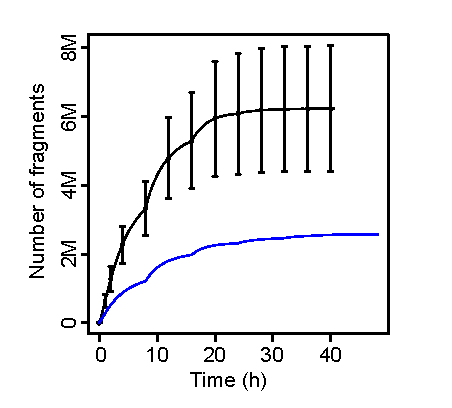
\includegraphics{frag_time.pdf}
\caption[SMURF-seq generates fragments at a faster rate than
  sequencing short molecules directly.]{
  SMURF-seq generates fragments at a faster rate than sequencing
  short molecules directly. Number of fragments obtained from reads
  plotted as a function of  sequencing time. For SMURF-seq, the average
  number of fragments from runs using the 1D sequencing by ligation kits
  are plotted (Error bars indicate one standard deviation). For short-read
  sequencing run, each read is considered as one fragment.}
\label{frag_time}
\end{figure}

%% Why does SMURF-seq perform better?
% pore reload time
The most important factor in the performance of SMURF-seq over
sequencing short molecules directly is that sequencing concatenated
fragments effectively eliminates the pore reload time for all but the
first fragment in each read. However, there are a variety of additional
factors that favor further optimization of the approach employed by
SMURF-seq.
% sequences fewer technical bases
First, reduction of resources spent on technical nucleotides: SMURF-seq
uses a single barcode and sequencing adapter per read consisting of
multiple fragments; sequencing short reads uses one barcode and adapter
per fragment, adding approximately 50 bases to each fragment. This
increases the time to sequence each short read. In sequencing short
reads, as the reads get shorter the time consumed by these technical
bases increases. In SMURF-seq, sequencing either shorter fragments in
fixed length reads, or longer reads containing fragments of fixed
average length, both reduce the time consumed sequencing these technical
bases.
%
In the limit, assuming 100bp DNA fragments, sequencing those fragments
as short-reads corresponds to 33\% technical nucleotides; for SMURF-seq,
the portion of technical nucleotides remains low.
% Nanopores sequence at full speed
Second, more nucleotides sequenced at full speed: We observed that the
speed of sequencing was lower when sequencing short molecules. For
example, the average sequencing speed was 315.54 bases per second for
sequencing the diploid genome without SMURF-seq, and 400.29 bases per
second when sequencing using SMURF-seq on the MinION sequencer.
% Compatible with all library prep kits
Third, leveraging optimizations to long-read protocols: The rapidly
evolving nanopore library construction kits are continually optimized
for long-read sequencing, and would likely require significant ad-hoc
modifications to optimize sequencing of short molecules of length
optimal for read-counting applications.


%%%%%%%%%%%%%%%%%%%%%%%%%%%%%%%%%%%%%%%%%%%%%%%%%%%%%%%%%%%%%%%%%%%%%%%%
%%%%%%%%%%%%%%%%%%%%%%%%%%%%%%%%%%%%%%%%%%%%%%%%%%%%%%%%%%%%%%%%%%%%%%%%
%%%%%%%%%%%%%%%%%%%%%%%%%%%%%%%%%%%%%%%%%%%%%%%%%%%%%%%%%%%%%%%%%%%%%%%%
\section{Efficient CNV profiling using SMURF-seq}
To demonstrate the utility of SMURF-seq, we generated CNV profiles of
normal diploid and highly rearranged cancer genomes.  The mapped
fragments were grouped into variable length ``bins'' across the genome
and bin counts were used to generate CNV profiles as described in
\citep{baslan2012genome,kendall2014computational}.

\subsection{Accurate CNV profiles using SMURF-seq}
\begin{figure}[b!]
\centering
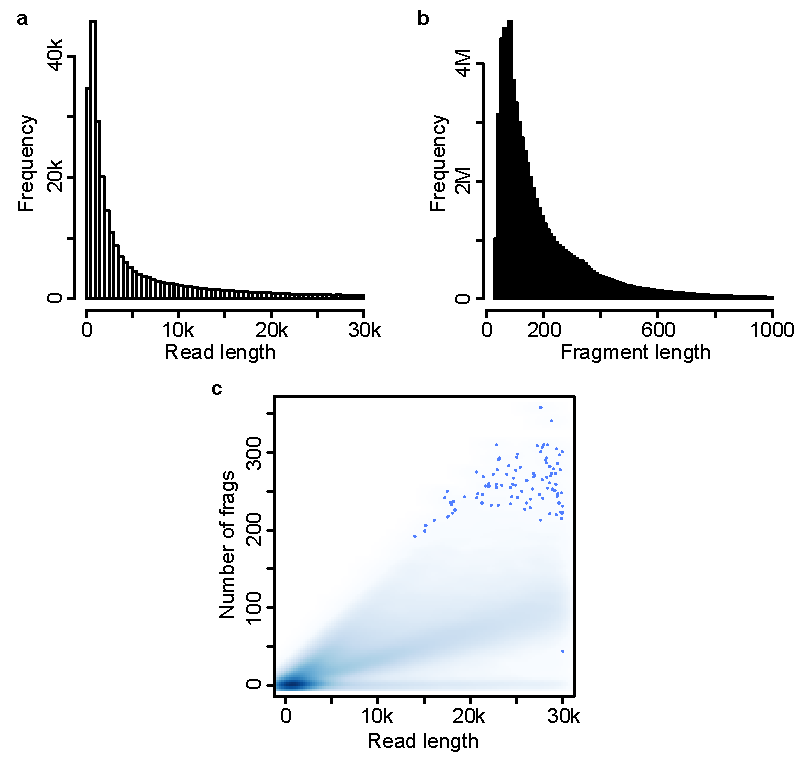
\includegraphics{read_frag_dist.pdf}
\caption[Read and fragment lengths from a SMURF-seq sequencing run.]{
  Read and fragment lengths from a SMURF-seq sequencing run.
  (a) Sequenced read length distribution.
  (b) Mapped fragment length distribution.
  (c) Scatter plot of read length and the number of fragments contained
  in the read.}
\label{read_frag_dist}
\end{figure}

%% Diploid genome
We sequenced a normal diploid female genome with SMURF-seq, resulting in
270.8k reads (mean read length of 6.75 kb) in a single run. These reads
were split into 7.28 million fragments (26.87 mean fragments per read;
Fig.~\ref{read_frag_dist}).
A CNV profile for this normal diploid genome, with the expected
(approximately flat) appearance can be seen in Fig.~\ref{cnv}a.
% Replicate
A replicate of this experiment resulted in 497.9k reads (mean read
length of 3.7 kb), which were split into 7.55 million fragments (15.16
mean fragments per read).

%% Rapid kit
The Rapid sequencing kit form Oxford Nanopore Technologies offers an
extremely fast (10 minute) and simple (2 step) protocol for library
preparation. We verified that the SMURF-seq procedure behaves similarly
using the Rapid Sequencing Kit. The 213.38k sequenced reads had a mean
read length of 3.9 kb, and were split into 2.81 million fragments.

%% skbr3 genome
Next we applied SMURF-seq to the breast cancer line SK-BR-3, generating
147.0k reads with mean length of 7.62 kb, which were split into 4.52
million fragments (30.78 mean fragments per read). We then obtained a
CNV profile using 5,000 bins, corresponding to an average bin size of
approximately 600 kb (Fig.~\ref{cnv}b).

\begin{figure}[b!]
\centering
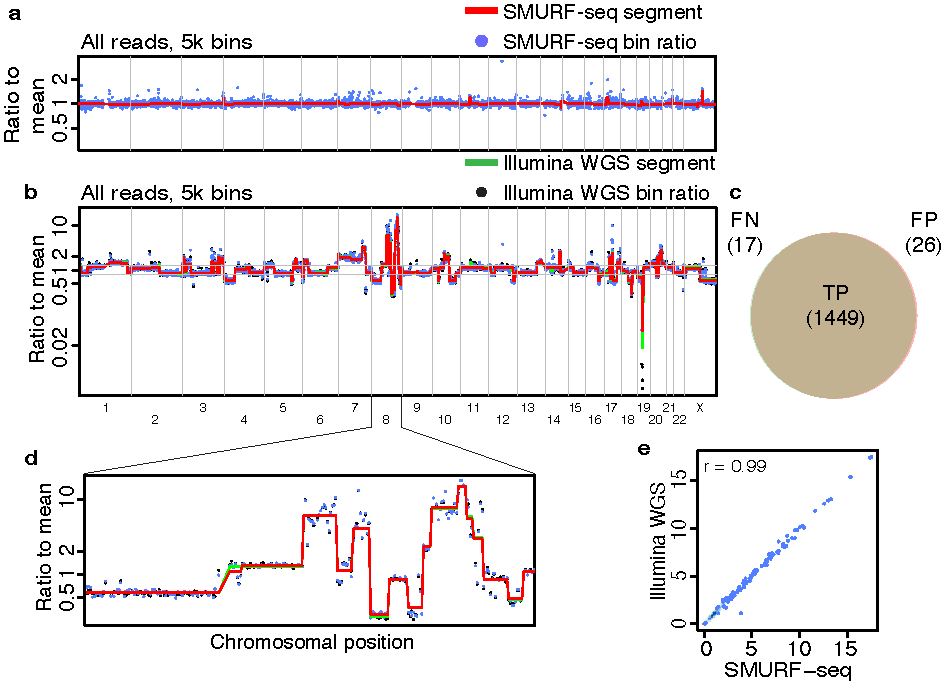
\includegraphics{ch3_fig4.pdf}
\caption[Accurate copy number profiles with SMURF-seq.]{
  Accurate copy number profiles with SMURF-seq.
  (a) CNV profile of a normal diploid genome. Each blue point is a
  bin ratio to mean and the red line is the segmented bin ratio.
  (b) Superimposed CNV profiles of SK-BR-3 genome generated using
  SMURF-seq and Illumina WGS reads.
  (c) Venn diagram illustrating the accuracy of event calls using
  SMURF-seq compared with Illumina WGS.
  (d) Zoom-in of copy number changes on chromosome 8.
  (e) Scatter plot of bin ratio of SK-BR-3 genome using
  SMURF-seq and Illumina WGS reads. Pearson correlation of the data
  is shown.}
\label{cnv}
\end{figure}

To provide a quantification of accuracy in terms of individual CNV
events we conducted whole-genome sequencing (WGS) on the same SK-BR-3
using Illumina (5.56 million reads; 130 bp, single-end).  We used this
to define a ground truth by calling CNV events for each of the
pre-defined bins (both amplifications and deletions) based on segmented
signal with a cutoff of 1.25/0.8 (Fig.~\ref{cnv}b)
\citep{dago2014rapid,berry2017potential}. This resulted in 1,466 events
(886 amplifications, 580 deletions) from 4,953 bins. We then called
events using the identical procedure with SMURF-seq data from the same
SK-BR-3 sample. The precision and recall for SMURF-seq relative to the
Illumina calls was 0.982 and 0.988, respectively (Fig.~\ref{cnv}c).
Fig.~\ref{cnv}d shows a zoom-in of a region with extreme copy number
alterations. The bin ratios for the Illumina WGS and the SMURF-seq
profiles are highly correlated (Pearson $r$ = 0.99; Fig.~\ref{cnv}e).
% replicate
A replicate of this experiment resulted 132.64k reads (mean read length
of 7.3 kb), which were split into 4.02 million fragments (30.31 mean
fragments per read).

\begin{figure}[t!]
\centering
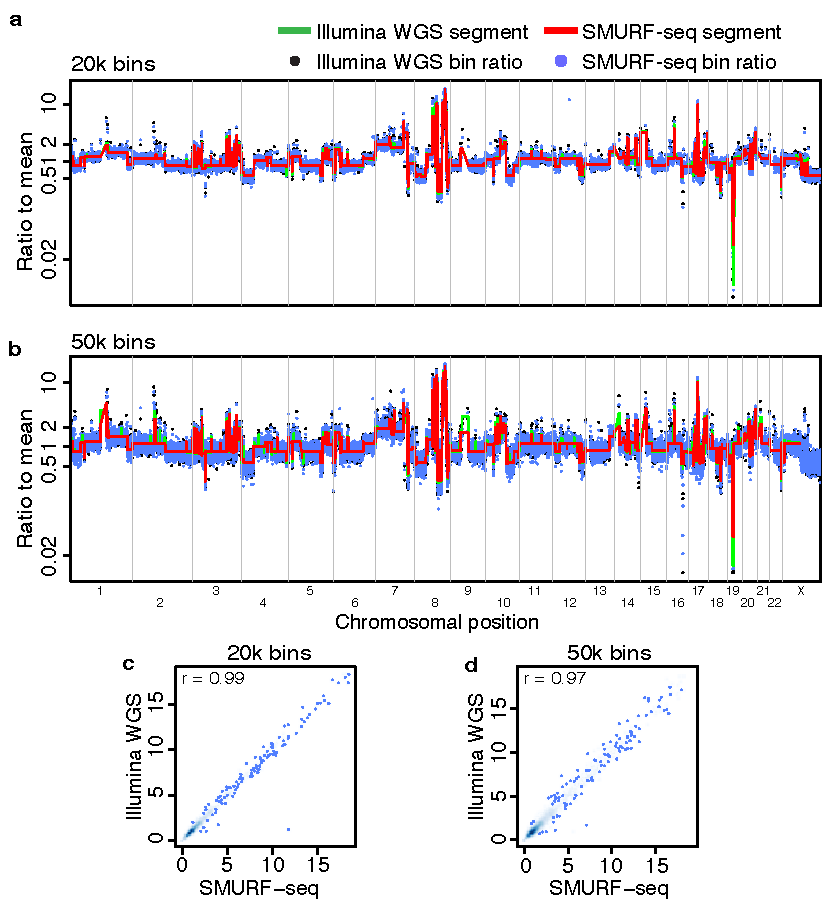
\includegraphics{skbr3_hi_res.pdf}
\caption[High resolution CNV profile with SMURF-seq]{
  High resolution CNV profile generated using SMURF-seq is highly concordant
  with the profile generated with Illumina WGS.
  (a, b) Superimposed CNV profiles of SK-BR-3 genome generated using SMURF-seq
  and Illumina WGS at 20,000 and 50,000 bin resolutions.
  (c, d) Scatter plot of bin ratios of SK-BR-3 genome using
  SMURF-seq and Illumina WGS reads at 20,000 and 50,000 bin resolutions. }
  \label{skbr3_hi_res}
\end{figure}

%% Hige resolution profiles
We also generated higher-resolution CNV profiles at 20,000 and 50,000
bins, corresponding to an average of approximately 150 kb and 60 kb in
length respectively (Fig.~\ref{skbr3_hi_res}a, b). The profiles obtained
at these resolutions have a high correlation with the profiles obtained
using Illumina WGS (Pearson $r>$ 0.97; Fig.~\ref{skbr3_hi_res}c, d).



\subsection{Concordant profiles from fewer countable fragments}
\begin{figure}[t!]
\centering
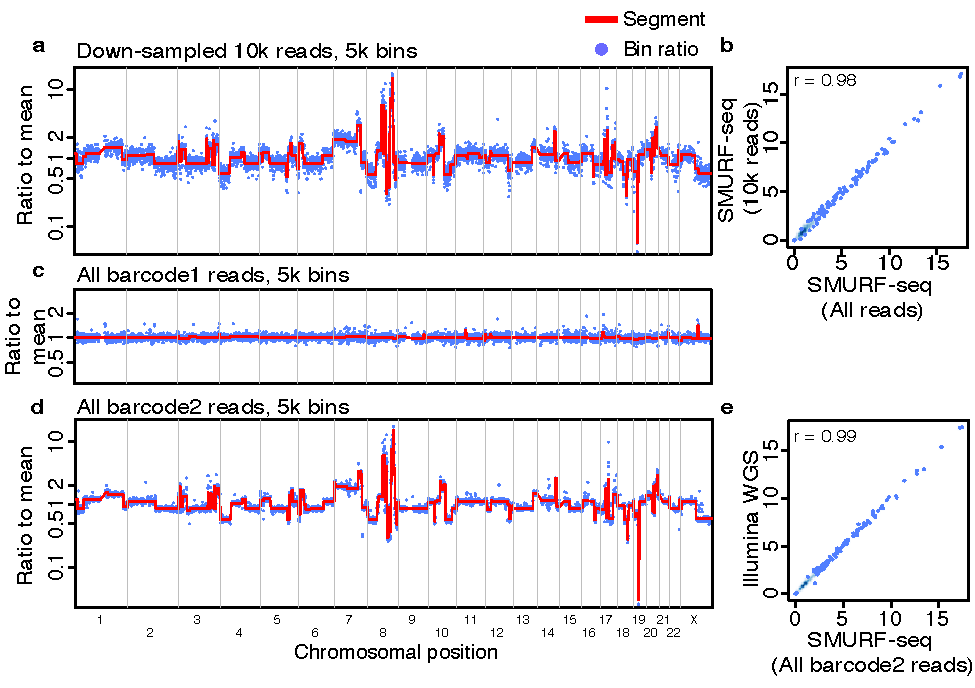
\includegraphics{ch3_fig5.pdf}
\caption[Multiple SMURF-seq CNV profiles by multiplexing in a single run]{
  Multiple SMURF-seq CNV profiles by multiplexing in a single run.
  (a) CNV profile of SK-BR-3 genome with down-sampled 10k SMURF-seq reads.
  (b) Scatter plot of normalized bin counts of the original SMURF-seq
  data and data down-sampled to 10k SMURF-seq reads. Pearson
  correlation of the data is shown.
  (c) CNV profile of barcode01 (Normal diploid genome) reads.
  (d) CNV profile of barcode02 (SK-BR-3 cancer genome) reads.
  (e) Scatter plot of bin ratios of SK-BR-3 genome using
  multiplexed SMURF-seq and Illumina WGS reads.}
\label{cnv_mux}
\end{figure}

Several cancer-related studies have employed CNV profiling based on
low-coverage WGS \citep{macintyre2018copy,kader2016copy}.  It has
previously been demonstrated that 250k reads are sufficient for accurate
genome-wide CNV profiling of single cells \citep{baslan2015optimizing}.
At the same time, the CNV profiles from a population of cells has been
shown to have a high correlation with single-cell profiles
\citep{navin2011tumour,baslan2015optimizing}. We reasoned that using 250k
fragments for CNV profiling using a population of cells would give
useful profiles if they remained sufficiently accurate.  By
down-sampling our SMURF-seq data, we verified that 10k reads,
approximately 250k fragments, result in highly-correlated CNV profiles
(Pearson $r$ = 0.98; Fig.~\ref{cnv_mux}a, b).

Given the total capacity of the MinION instrument, this indicates that
multiple samples can effectively be barcoded and multiplexed in a single
sequencing run.
%%
To verify this we sequenced two DNA samples (normal diploid female and
SK-BR-3) in a single run.  These samples were processed with SMURF-seq
protocol and then barcoded following the standard library construction.
After demultiplexing and mapping the reads, the diploid genome had a CNV
profile as expected (Fig.~\ref{cnv_mux}c) and the SK-BR-3 CNV profile
was nearly identical to the profile obtained using Illumina WGS (Pearson
$r$ = 0.99; Fig.~\ref{cnv_mux}d, e). All the sequencing runs and the
availability of sequence data is summarized in Appendix~\ref{appendB}.

\begin{figure}[t!]
\centering
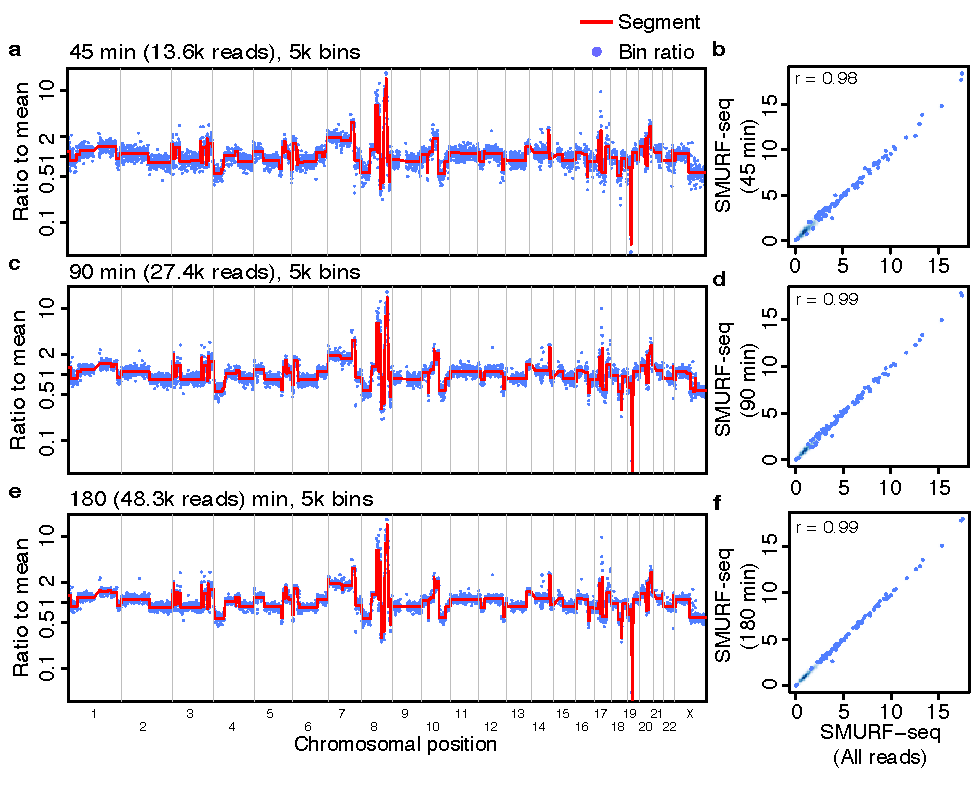
\includegraphics{cnv_time.pdf}
\caption[CNV profile with reads obtained in first few minutes of
  sequencing]{
  CNV profile with reads obtained in first few minutes of sequencing.
  (a, c, e) CNV profile  with reads obtained in the first 45, 90,
  and 180 minutes of sequencing.
  (b, d, f) Scatter plot of bin ratios of the original
  SMURF-seq data and data obtained in first 45, 90, and 180
  minutes of sequencing.}
  \label{cnv_time}
\end{figure}

%% Terminating sequencing early
Further, we verified that the CNV profile with reads generated in the
first 45, 90, and 180 minutes of starting a sequencing run had a high
correlation to the profile with reads from the complete run (Pearson $r>$
0.98; Fig.~\ref{cnv_time}).

In summary, our results demonstrate that SMURF-seq can generate more
information for CNV analysis in a single run of the Oxford MinION
sequencer, compared with either producing long reads in the usual way or
direct short-read sequencing on the same instrument.  This increased
information is in the form of increased numbers of distinct DNA
fragments sequenced, and can be leveraged in multiple ways. Applying
SMURF-seq on a single sample for a full run corresponds to higher counts
for downstream analysis. In CNV analysis, increased counts either add
confidence for a fixed resolution, or can allow higher resolution
analysis (i.e. smaller bins) at the same level of confidence.
Alternatively, the increased information throughput can effectively
reduce the time required to produce the same number of counts for CNV
analysis by terminating the sequencing earlier. Finally, the increased
information yield can be directed towards reducing the cost of
generating CNV profiles by allowing a greater degree of multiplexing.
For CNV analysis at resolutions permitted by 250k mapped fragments, our
results show SMURF-seq allows roughly 20 and up to 30 samples in a
single run, compared with 10 per run directly using short-read
sequencing.

%%%%%%%%%%%%%%%%%%%%%%%%%%%%%%%%%%%%%%%%%%%%%%%%%%%%%%%%%%%%%%%%%%%%%%%%
%%%%%%%%%%%%%%%%%%%%%%%%%%%%%%%%%%%%%%%%%%%%%%%%%%%%%%%%%%%%%%%%%%%%%%%%
%%%%%%%%%%%%%%%%%%%%%%%%%%%%%%%%%%%%%%%%%%%%%%%%%%%%%%%%%%%%%%%%%%%%%%%%
\section{Future of SMURF-seq}

